\fontsize{13px}{13px}\selectfont\justifying

\section{Phân tích, thiết kế}\label{section:readme}
	\begin{figure}[h!]\fontsize{13px}{13px}\selectfont
		\begin{center}	
			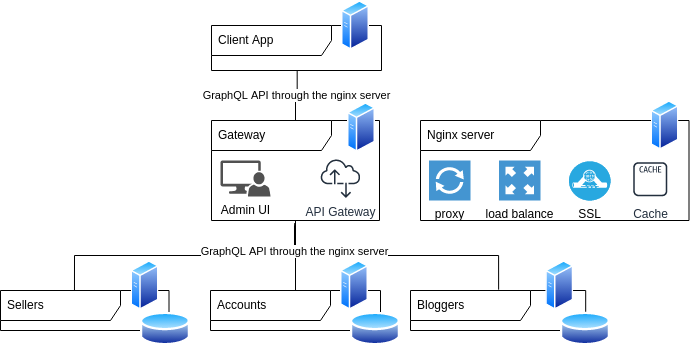
\includegraphics[width=\textwidth]{srs}
			\caption{Thiết kế chung của hệ thống}
		\end{center}
	\end{figure}
	Hệ thống thiết kế hướng dịch vụ chia làm 3 dịch vụ nhỏ là: sellers, accounts và bloggers. Tại máy chủ gateway có nhiệm vụ phân tích truy vấn đồ thị thành nhiều đồ thị con và gửi đến các dịch vụ xử lý. Sau đó gộp kết quả lại và trả về cho truy vấn. Gateway đồng thời cũng cung cấp giao diện quản lý chung cho tất cả các dịch vụ.
	
	Giao tiếp giữa các máy chủ dịch vụ thực hiện thông qua phương thức \acrshort{http}. Sử dụng máy chủ web nginx để liên kết cổng. Đồng thời thực hiện các chức năng chứng thực, phân phối tải,...